\section{Mô hình đa chiều và Data Dictionary}
\subsection{Grain và mô hình vật lý}
Tên cột, kiểu, nullable và ràng buộc dưới đây lấy từ DDL của kho (\code{sql/dw/dw_schema.sql}) và của staging (\code{sql/staging/01_schema.sql}).

\code{dw.fact_sales} có grain một cặp (order\_id, order\_item\_id), với PK ghép đúng hai cột đó. Một sản phẩm có thể xuất hiện ở nhiều dòng cùng đơn nên grain không phải cặp (order, product). Hai measure vật lý là \code{price} và \code{freight_value}, kiểu \code{NUMERIC(10,2)}, NOT NULL và có CHECK không âm. Số món được tính bằng COUNT(*) trên các dòng hàng.

\code{dw.fact_customer_order} có grain một order\_id, giữ toàn bộ trạng thái, ngày mua, ngày duyệt, địa lý khách tại đơn và tổng thanh toán. \code{total_payment_value} là \code{NUMERIC(12,2)}, cho phép NULL; điều kiện CHECK chỉ chặn giá trị âm. Thanh toán được cộng theo đơn trước khi nối với fact, nhờ đó tránh tích chéo giữa nhiều dòng hàng và nhiều dòng thanh toán.

Mô hình là chòm sao fact (fact constellation) \cite{kimball} với dimension dùng chung, đồng thời có FK từ fact sales đến fact đơn. Đây không phải một Star Schema đơn lẻ độc lập, cũng không phải snowflake vì không có bảng dimension con. Sơ đồ hình~\ref{fig:physical} phản ánh nguyên trạng DDL, gồm cả cạnh fact--fact.

\begin{table}[H]\centering\small\renewcommand{\arraystretch}{1.15}
\begin{tabularx}{\linewidth}{p{3cm}YY}
\toprule Bảng dimension & Grain và khóa & Thuộc tính / vai trò\\\midrule
\code{dim_date} & Một ngày; PK date\_key=YYYYMMDD; full\_date UNIQUE & Năm, quý, tháng, ngày, thứ ISO, cuối tuần. Hai vai trò mua và duyệt.\\
\code{dim_customer} & Một customer\_unique\_id; customer\_key SERIAL PK & Business key CHAR(32), NOT NULL UNIQUE; không giữ thành phố/bang.\\
\code{dim_product} & Một product\_id; product\_key SERIAL PK & Business key CHAR(32), NOT NULL UNIQUE; danh mục gốc/Anh nullable.\\
\code{dim_seller} & Một seller\_id; seller\_key SERIAL PK & Business key CHAR(32), NOT NULL UNIQUE; không có địa lý seller.\\
\bottomrule\end{tabularx}
\caption{Các bảng dimension}
\end{table}

% Giữ trang sơ đồ ở khổ dọc theo yêu cầu, chấp nhận chữ trong hình nhỏ.
\clearpage
\begin{figure}[p]\centering
\sbox0{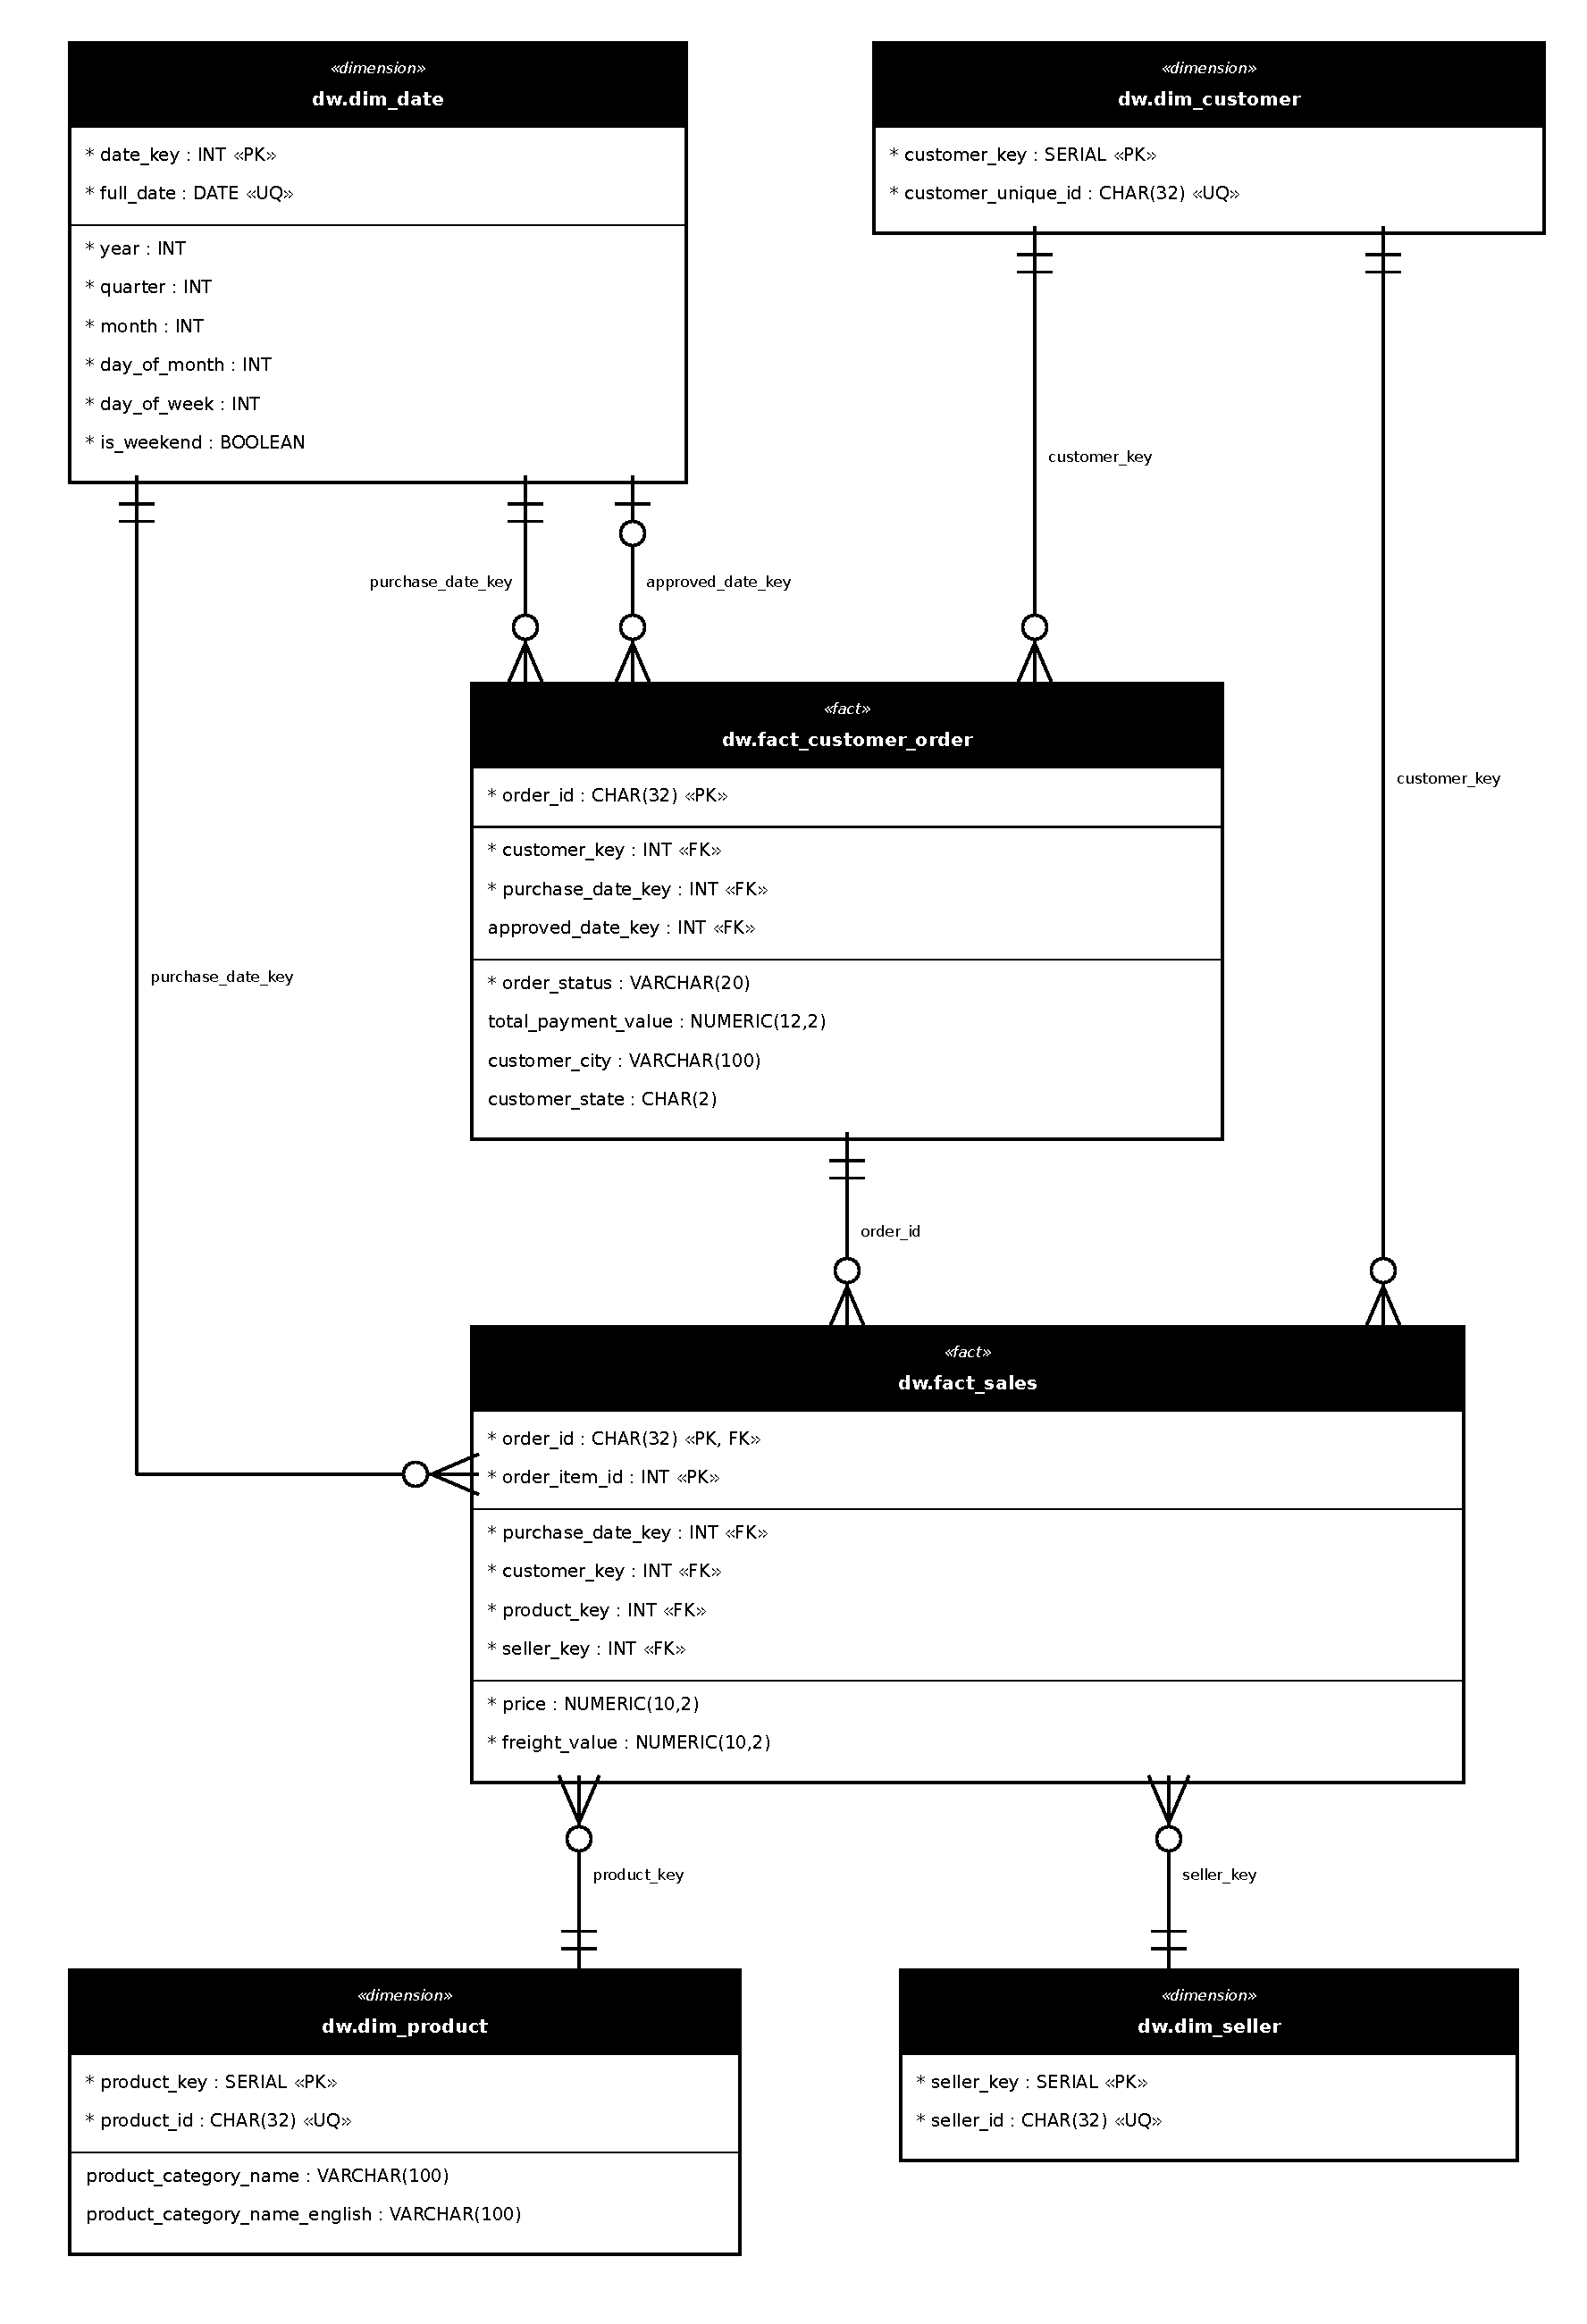
\includegraphics[width=\linewidth,height=0.83\textheight,keepaspectratio]{assets/fig_star_schema.pdf}}%
\setlength{\unitlength}{\wd0}%
\begin{picture}(1,1.4646)
\put(0,0){\usebox0}
\put(0.567,0.045){\sffamily\scriptsize Dấu * biểu diễn NOT NULL.}
\end{picture}
\caption{Mô hình vật lý của kho dữ liệu}
\label{fig:physical}
\end{figure}
\clearpage

\subsection{Quan hệ và khả năng cộng gộp}
Tất cả quan hệ DW là một--nhiều từ dimension sang fact, hoặc từ fact đơn sang fact sales. Mỗi dòng con có đúng một cha nếu FK bắt buộc; riêng \code{approved_date_key} nullable nên có 0 hoặc 1 ngày duyệt. DDL không bắt buộc một cha phải có ít nhất một con nên cardinality phía dòng con luôn là 0..N. Thực tế CSV có 775 đơn chưa có dòng hàng.

\code{purchase_date_key} và \code{customer_key} xuất hiện ở cả hai fact. Các FK riêng lẻ không tự bảo đảm chúng trùng khớp trên cùng \code{order_id}; script validate mới kiểm tra điều kiện này. Kho không dùng SCD Type 2, cột hiệu lực, thành viên ``unknown'' hay nạp tăng dần. Khóa SERIAL được sinh khi nạp nên không dùng làm định danh nghiệp vụ.

Tiền hàng và cước cộng được theo các chiều tại grain dòng sản phẩm. Tổng thanh toán chỉ cộng ở grain đơn hoặc sau khi gom mỗi đơn một lần; nối fact đơn với fact sales rồi SUM(total\_payment\_value) sẽ nhân bản tiền theo số dòng hàng. Số đơn riêng biệt không cộng được xuyên danh mục/seller; số khách riêng biệt không cộng được xuyên bang/năm. AOV và tỷ lệ phải tính lại từ tử số và mẫu số, không lấy trung bình đơn giản của các trung bình. Khi cần trạng thái hoặc địa lý đơn cho phân tích ở grain dòng hàng, truy vấn OLAP nối \code{fact_sales} với \code{fact_customer_order} trên \code{order_id} (quan hệ nhiều--một, không nhân bản dòng); các API màn Thời gian dùng phép nối này để lọc đơn delivered.

\subsection{Từ điển dữ liệu}
\begin{table}[H]\centering\small\renewcommand{\arraystretch}{1.1}
\begin{tabularx}{\linewidth}{p{3.5cm}p{2.9cm}Y}
\toprule Cột & Kiểu & Ý nghĩa\\\midrule
\multicolumn{3}{l}{dw.fact\_sales -- PK (order\_id, order\_item\_id)}\\
\code{order_id}, \code{order_item_id} & CHAR(32), INT & Định danh dòng hàng; FK \code{order_id} tới fact đơn.\\
\code{purchase_date_key} & INT & FK \code{dim_date}, ngày mua.\\
\code{customer_key}, \code{product_key}, \code{seller_key} & INT & FK tới ba dimension.\\
\code{price}, \code{freight_value} & NUMERIC(10,2) & Tiền hàng và cước của dòng; NOT NULL, $\geq 0$.\\
\midrule
\multicolumn{3}{l}{dw.fact\_customer\_order -- PK order\_id}\\
\code{customer_key} & INT & FK \code{dim_customer}.\\
\code{purchase_date_key}, \code{approved_date_key} & INT & FK \code{dim_date}; ngày duyệt có thể NULL.\\
\code{order_status} & VARCHAR(20) & Trạng thái đơn.\\
\code{total_payment_value} & NUMERIC(12,2) & Tổng thanh toán của đơn; NULL nếu không có dòng thanh toán, $\geq 0$.\\
\code{customer_city}, \code{customer_state} & VARCHAR, CHAR(2) & Địa lý khách tại thời điểm đặt đơn.\\
\bottomrule\end{tabularx}
\caption{Từ điển dữ liệu bảng fact}
\end{table}

Tầng raw giữ toàn bộ cột CSV kiểu TEXT, không khóa. Tầng staging có kiểu, PK/FK và chỉ giữ thuộc tính cần cho phân tích. Dữ liệu không có thông tin múi giờ nghiệp vụ nên ngày được lấy theo giá trị trong CSV.
